\chapter{Software}
\label{Chapter3}
O \ac{ide} utilizado neste trabalho foi o \textbf{\textit{{Microchip Studio for AVR\textsuperscript{\textregistered} and SAM Devices}}} (\textit{version: 7.0.2542}). A programação foi feita em Linguagem \textbf{C}, sua estrutura sintática esta abaixo mencionado:
\\
\\
\begin{figure}[H]
	\centering
	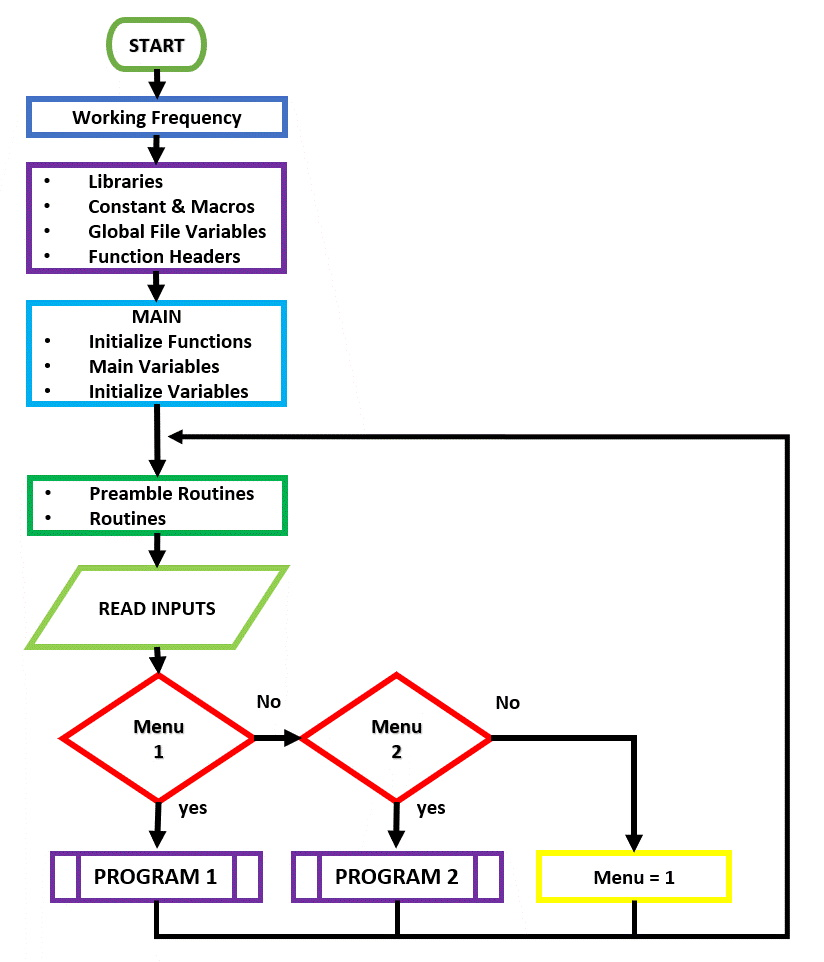
\includegraphics[scale=0.6]{./image/PESTA/flowchart/Main_Program_1.jpg}
	\caption{Estrutura do Programa (fluxograma)}
	\label{Main_Program_1}
\end{figure}
\figurespace{.5}
O \textit{PROGRAM 1} é onde corre o programa da balança, e o \textit{PROGRAM 2} usado para calibração do \textit{Gain Factor}.
\\
\\
Todos os programas sequem uma estrutura sintática recursiva usando o seguinte modelo.
\\
\\
\begin{figure}[H]
	\centering
	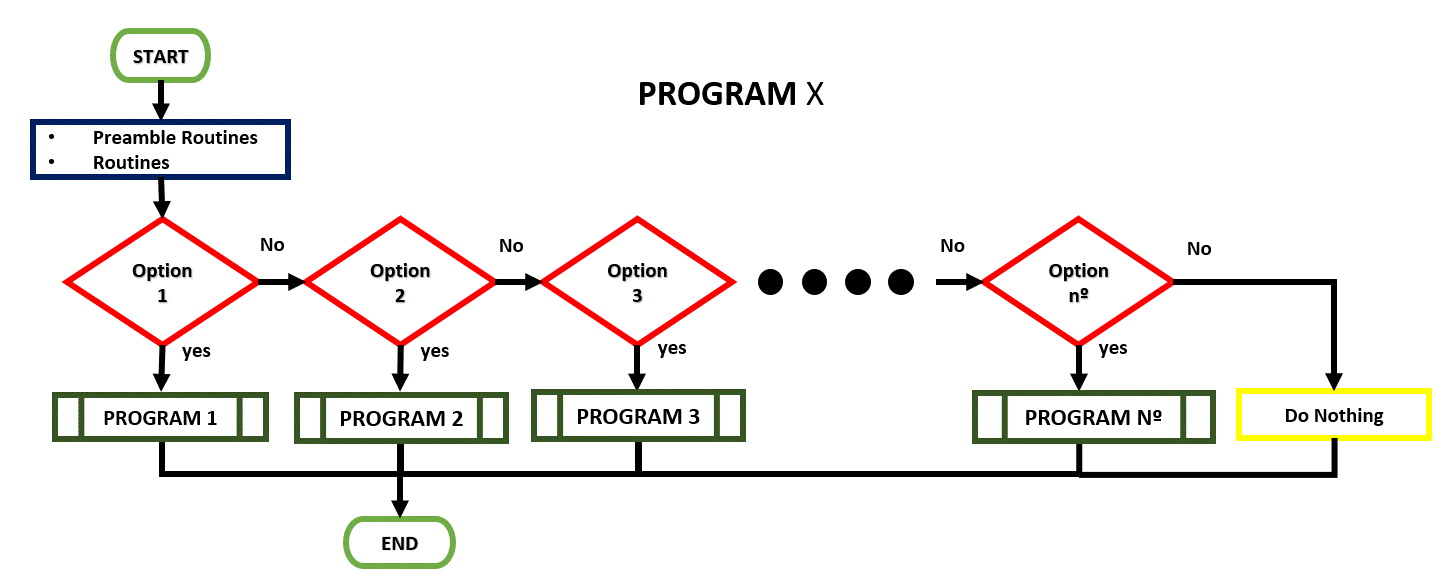
\includegraphics[scale=0.40]{./image/PESTA/flowchart/Generic_structure.jpg}
	\caption{Sintaxe Genérica dos programas (fluxograma)}
	\label{Geneic_structure}
\end{figure}
\figurespace{.5}
Duas interrupções periódicas estão sempre a correr em \textit{background}, uma para fazer o \textit{shift} dos \textit{bit´s} da conversão \textbf{ADC} feita pelo amplificador de sinal HX711 e outra interrupção periódica de segundo em segundo usado para saltar de \textit{Menu} pelos botões.
\\
\\
\begin{minipage}{\linewidth}
	\begin{minipage}{.5\linewidth}
		\begin{figure}[H]
			\centering
			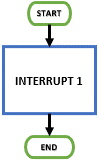
\includegraphics[scale=0.7]{./image/PESTA/flowchart/Interrupt_1.jpg}
			\caption{\textbf{ADC} conversão}
			\label{Interrupt_1}
		\end{figure}
	\end{minipage}
	\begin{minipage}{.5\linewidth}
		\begin{figure}[H]
			\centering
			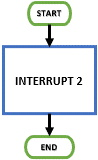
\includegraphics[scale=0.7]{./image/PESTA/flowchart/Interrupt_2.jpg}
			\caption{Saltar de \textit{Menu}}
			\label{Interrupt_2}
		\end{figure}
	\end{minipage}
\end{minipage}
\minipagespace{.5}
Consultar código para leitura das rotinas de interrupção nas folhas \textit{anexas}.
\\
\\
\begin{minipage}{.40\linewidth}
	\begin{figure}[H]
		\flushleft
		\captionsetup{justification=raggedright,singlelinecheck=false}
		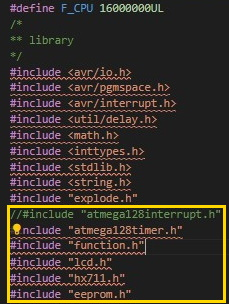
\includegraphics[scale=0.9]{./image/PESTA/Code/Livrarias.jpg}
		\caption{Livrarias}
		\label{Livrarias}
	\end{figure}
\end{minipage}
\begin{minipage}{.6\linewidth}
	Ao lado esta as livrarias usadas neste projeto, as que estão dentro da caixa amarela são as que foram criadas.
	A filosofia usada é de criar objetos que representam o hardware para o poder manipular via código. Como se pode observar foi criado uma livraria para os temporizadores, outra para as interrupções e \ac{eeprom}, depois criado livrarias para os componentes externos, isto é, o \textbf{LCD} e o integrado \textbf{HX711}. \\
	Uma abstração que torna simples executar qualquer algoritmo ou projeto, e isto só é possível depois de ultrapassar a barreira árdua e dolorosa de desenvolver as livrarias.
	\\
	\\
	\\
\end{minipage}
\minipagespace{.5}
Durante este projeto tentou-se dentro do possível sempre seguir as boas praticas de programação, como a \texttt{indentação} especifica para cada situação, e manter a estrutura de norma. Deve-se manter uma metodologia de trabalho que segue as normas assim é percetível para todos e facilita detetar \textit{bugs}, e é uma pratica que abrange todas as linguagens, por exemplo o \textbf{Python} é fundado nesse principio.
\\
\\
Quanto as interrupções é sempre um desafio, porque as tarefas tem que ser bem organizadas temporalmente para não entrar em conflitos, pretende-se assim sempre que o código corra na função \textit{main} e as interrupções algo esporádico e muito rápido, estas devem servir de \textit{flags} para executar rotinas na função \textit{main}, ou seja, servirem de \textbf{\textcolor{green}{INPUTS}}.
\newpage
\section{Validação}
%%%To validate is to justify why the choices made and alternatives that could be chosen.
As escolhas feitas estão dentro dos parâmetros da oferta disponibilizada. Apenas o conhecimento adquirido ao aprofundar o funcionamento dos componentes é o ganho mais evidente, facilitando a interpretação de situações e deteção de anomalias (\textit{troubleshooting}), derivado aos custos dos materiais serem caros.\\
\\
Apostei na marca \textbf{Atmel} devido a experiência e conhecimentos já adquiridos, se aposta-se noutra marca teria de enfrentar uma curva de aprendizagem e adaptação que no final a nível de custos beneficio seria desfavorável, pelo tempo a dispensar e de ser muito trabalhoso a refazer tudo novamente noutra arquitetura.\\
\\
O sensor usado é o mais comum nesta pratica, e escolha demonstrada, o circuito de interface é indiferente a escolha apenas é baseada na sua precisão, ou seja, é de \textcolor{blue}{24} \textit{bit} enquanto o \textbf{ADC} do \textbf{MCU} de \textcolor{blue}{10} \textit{bit}.
\\
\\
\\
\subsection{Material}
Abaixo esta indicado uma tabela dos materiais usados, assim como os preços.
\\
\\
\begin{table}[H]{
		\caption{Lista de material}
		\rowcolors{3}{blue!80!yellow!50}{blue!70!yellow!40}
		\begin{tabular}{ |p{12cm}|c|p{2cm}|  }
			\hline
			\multicolumn{3}{|c|}{Lista de Material} \\
			\hline
			Peça & Quant & Preço [uni] \\
			\hline
			Fonte de alimetação 12V 1A & 1 & \EUR{3.87} \\
			Conversor DC-DC com voltímetro & 1 & \EUR{7.75} \\
			ET BASE AVR Atmega128 Board & 1 & \EUR{23.92} \\
			Test Input Board  & 1 & \EUR{3.71} \\
			Test Output Board & 1 & \EUR{3.71} \\
			IDC Socket 10 way    & 12 & \EUR{0.31} \\
			IDC Header Straight 10 way    & 12 & \EUR{0.25} \\
			Flatcable    & ? & \EUR{?} \\
			20x4 LCD Module Blue & 1 & \EUR{12.24} \\
			SparkFun Load Cell Amplifier HX711 & 1 & \EUR{13.04}   \\
			50Kg Load Cell & 1 & \EUR{12} \\
			\hline
			& \textit{total} & \EUR{86.96} \\
			\hline
		\end{tabular}
	}
	\label{material}
\end{table}
\newpage
\subsection{Testar}
Quanto a funcionalidade no seu todo a balança tem \textcolor{blue}{quatro} botões e \textcolor{blue}{três} \textit{leds} ativados, um botão para fazer o \textit{offset} no \textcolor{green}{PORTF 0}, e dois botões com dupla função, fazer \textit{reset} para \textit{default} e incrementar, outro para entrar no menu de calibração e decrementar, o \textcolor{blue}{quarto} botão é reservado para \textit{enter} e assumir o valor introduzido na calibração.\\
\\
O botão \textcolor{green}{PORTF 3} quando premido durante \textcolor{blue}{cinco} segundos faz um \textit{reset} para configuração \textit{default} depois de o \textit{led} no \textcolor{red}{PORTC 6} piscar \textcolor{blue}{quatro} vezes.\\
\\
O botão \textcolor{green}{PORTF 4} quando premido durante \textcolor{blue}{cinco} segundos entra no menu de calibração do valor do \textit{gain factor} e o \textit{led} no \textcolor{red}{PORTC 7} liga, usando os botões de incrementa e decrementar, isto é, o
\textcolor{green}{PORTF 3} e \textcolor{green}{PORTF 4} pode-se alterar esse valor.\\
\\
Para assumir o valor e sair do menu de calibração basta premir o botão colocado no \textcolor{green}{PORTF 5}. Tanto no caso de calibração ou de \textit{offset} os valores são guardados na \textbf{EEPROM} do microcontrolador, sendo que, se retirar a alimentação do circuito este não perde os valores e o \textit{led} \textcolor{red}{PORTC 5} permanece ligado.
\\
\\
%%%%%%%%%%%%%%%%%%%%%%%%%%%%%%%%%%%%%%%%%%%%%%%%%%%%%%%%%%%%%%%%
\begin{comment}
Sem contar com as despesas no equipamento para a programação do hardware que em principio só se gasta uma vez, isto é, se não se estragar. No caso do programador \textbf{Atmel-ICE} pode custar até \EUR{185.55}.\\
\\
É de ter em conta que os preços são \textbf{PVP}, que no caso se for preços comerciais são dez vezes inferior, e se for para produção em grande escala também tem descontos por quantidade.\\
$\begin{array}{l l l}
\text{Média} & & \\
\overline{x} & = & \frac{1}{n}\sum_{i=1}^n x_i
\end{array}$
MEMS devices and structures are fabricated using conventional integrated circuit process techniques, such as lithography, deposition, and etching, together with a broad range of specially developed micromachining techniques. \cite{book-9}
The three essential elements in conventional silicon processing are deposition, lithography, and etching. \cite{book-9}
Sensitivity,Long-Term Drift e Temperature Effects (Span temperature hysteresis).
\end{comment}
%%%%%%%%%%%%%%%%%%%%%%%%%%%%%%%%%%%%%%%%%%%%%%%%%%%%%%%%%%%%%%%%
